% REMEMBER: You must not plagiarise anything in your report. Be extremely careful.

\documentclass{l4proj}


%
% put any additional packages here
%
\usepackage{pgf-umlsd}
\usepackage{scalefnt}
\usepackage{tikz}

\begin{document}


%==============================================================================
%% METADATA
\title{Where Is ECN Stripped On the Network?}
\author{Myles Lamb}
\date{March 26, 2021}

\maketitle

%==============================================================================
%% ABSTRACT
\begin{abstract}
    % Every abstract follows a similar pattern. Motivate; set aims; describe work; explain results.
    % \vskip 0.5em
    % ``XYZ is bad. This project investigated ABC to determine if it was better. 
    % ABC used XXX and YYY to implement ZZZ. This is particularly interesting as XXX and YYY have
    % never been used together. It was found that  
    % ABC was 20\% better than XYZ, though it caused rabies in half of subjects.''
    
    This paper investigates where on the network ECT codepoints are removed by network devices, we investigate this through the production of a new network analysis tool, allowing for the observation of the modifications of packets on the network. We analyse three server three server populations under a variety of transport layer protocols.
\end{abstract}

%==============================================================================

% EDUCATION REUSE CONSENT FORM
% If you consent to your project being shown to future students for educational purposes
% then insert your name and the date below to  sign the education use form that appears in the front of the document. 
% You must explicitly give consent if you wish to do so.
% If you sign, your project may be included in the Hall of Fame if it scores particularly highly.
%
% Please note that you are under no obligation to sign 
% this declaration, but doing so would help future students.
%
\def\consentname {Myles Lamb} % your full name
\def\consentdate {26 March 2021} % the date you agree

\educationalconsent


%==============================================================================
\tableofcontents

%==============================================================================
%% Notes on formatting
%==============================================================================
% The first page, abstract and table of contents are numbered using Roman numerals and are not
% included in the page count. 
%
% From now on pages are numbered
% using Arabic numerals. Therefore, immediately after the first call to \chapter we need the call
% \pagenumbering{arabic} and this should be called once only in the document. 
%
% The first Chapter should then be on page 1. You are allowed 40 pages for a 40 credit project and 20 pages for a 
% 20 credit report. This includes everything numbered in Arabic numerals (excluding front matter) up
% to but excluding the appendices and bibliography.
%
% You must not alter text size (it is currently 10pt) or alter margins or spacing.
%
%
%==================================================================================================================================
%
% IMPORTANT
% The chapter headings here are **suggestions**. You don't have to follow this model if
% it doesn't fit your project. Every project should have an introduction and conclusion,
% however. 
%
%==================================================================================================================================
remove subsection
remove bullet points

background a little hard to follow

\chapter{Introduction}
\label{chap:introduction}

% reset page numbering. Don't remove this!
\pagenumbering{arabic} 

This chapter will motivate the development of a new network analysis tool, to investigate the adoption of Explicit Congestion Notification (ECN) and the frequency and location on the network where ECN expressions are altered by devices on the network path. Following chapters will go into detail, discussing various aspects of the project, such as the design and implementation of the network analysis tool and and evaluation of the results of a medium scale deployment of the previously developed tool.

\section{Motivation}

The deployment of ECN has been slowed due to issues relating to devices on the network dropping packets that attempt to utilise ECN, resetting connections that attempt to negoatiate ECN or remarking packets that indicate ECN capable transport (\cite{floyd_inappropriate_2002}), ultimately leading to a lack of faith in the technology. Whilst these issues have lessened in prevalence over time (\cite{trammell_enabling_2015}), there has been a renewed interest in the deployment of ECN through its integration with Quic, a new transport protocol operating over UDP (\cite{johansson_ecn_2017}), as well as the growing need to reduce queuing delay across modern networks, given the increasing prevalence of real time traffic, presenting the preservation of ECN markings across the network as critical for managing the continued development of the internet. To the best of our knowledge this paper presents first set of findings relating to the deployment of ECN within Quic. As well as presenting a new technical method for measuring on path removal of codepoints to TCP based hosts.

\section{Aim}

The aim of this paper is to investigate the overall adoption of ECN and how often, as well as where devices on the network modify the expression of ECN markings, serving as another datapoint of active ECN measurements over the last two decades. Additionally investigating whether choices of network substrate such as the Internet protocol version or transport layer substrate influence the modification patholgoies of ECN functionality, whether the ECT codepoint used influences the characteristics of the modfication of packets on the network. Lastly, evaluating ECN adoption and modification pathologies for Quic, a  new transport protocol implemented over UDP that has introduced support for ECN. To achieve this we will; Devise a suitable experimental methodology to gather appropriate measurements from the network (Section \ref{chap:design}), Design and implement a network analysis tool supporting the goals of the experimental methodology (Section \ref{chap:design} and Section \ref{chap:implementation}), Evaluate the network analysis tool through a medium scale deployment across numerous geographically distributed hosts (Section \ref{chap:evaluation}).

\clearpage


%==================================================================================================================================
\chapter{Background}

This chapter discusses the fundamentals of ECN as a technology and presents the contributions of previous works. Identifying areas for elaboration in existing research.
\addtocontents{toc}{\protect\setcounter{tocdepth}{1}}

\section{Overview of ECN}

The traditional, end to end approach to congestion control employed within transport protocols such as TCP results in end hosts inferring congestion on the network through signals such as packet loss.
ECN is a mechanism that allows for devices on the network to signal incipient congestion to end hosts before congestive loss occurs. This allows routers utilising Active Queue Management (ie. Random Early Detection) to mark packets when congestion is experienced. Receivers observing these markings inform the sender of their observation, allowing the sender to reduce their sending rate, before a congestive loss occurs. Potentially reducing negative aspects of loss based congestion signals such as, Head-of-line blocking for protocols that provide an in-order delivery service model such as TCP, or providing benefits to the quality of service for protocols that do not re-transmit lost packets such as RTP.

ECN is implemented through the 2 least significant bits of the traffic class byte of the IPv4/IPv6 header. These two bits of the IP header are used to signify whether a given transport is ECN capable, and whether congestion has been experienced on the network. We have four ECT (ECN capable transport) codepoints. 00 = not ECN capable, 10 = ECT(0), 01 = ECT(1), 11 = CE, or congestion experienced. 

It may be noted that both ECT(0) and ECT(1) are to be treated equivalently by devices on the network in identifying ECN capable transport (\cite{floyd_addition_2001}). Furthermore if a device on the network does not leverage the ECN field, it is not to modify it. Historically, the bits that constitute the ECN field occupy the same space as the legacy ToS (Type of Service) byte, providing some insight into why ECN is removed on the network, with some older equipment on the network continuing to use ToS semantics and subsequently erroneously clearing the ECN field (\cite{kuhlewind_state_2013}).

\subsection{Historic use of ToS and its implications}

As previously mentioned, the bits in the IP header that constitute the ECN field did not always serve this purpose, historically these bits constituted part of the Type of Service field. Which served many related purposes over the years of its use. Originally presented in RFC 792 and further updated in RFC 1583 it was primarily used to identify the precedence as well as providing mechanisms to request specific treatment on the network such as, low latency, or high reliability. However the latter was seldom used outside of a few specific use case scenarios. Whilst efforts were made to ensure some level of compatibility between ToS and the later introduced DSCP, such as maintaining the IP Precedence aspect of ToS. this could not be extended to ECN, The bits that constitute ECN where either unused as defied in RFC 792, or otherwise in RFC 1583 the rightmost bit was to always contain a value of zero. \cite{custura_exploring_2017} showed the existence of a number of devices on the internet that continue to use ToS based semantics, within a number of Autonomous Systems. exhibiting marking pathologies that are destructive towards ECN.
% Discuss research concerning the %

\section{ECN within TCP}



When ECN is utilised with TCP, hosts must first negotiate its use at the beginning of the TCP connection, during the SYN-ACK exchange. Utilising two, previously reserved bits of the TCP header. Namely the ECE (ECN Echo) and the CWR (Congestion window reduced) bits. Hosts may negotiate ECN through setting the ECE and CWR bits of the TCP header on the initiating SYN of the TCP handshake. If the receiving host also desires to use ECN, a SYN-ACK with the ECE bit set will be returned. Subsequent data segments sent during the connection should be marked with either ECT(0) or ECT(1) on the IP header to indicate ECN capable transport. Given when congestion is experienced on the network, and some device marks a given packet with the ECE codepoint. End hosts receiving a packet with the CE codepoint set should respond by setting the ECE bit on the following segment sent during the connection. The, sending host, then indicates the reciept of a segment with ECE bit, by setting the CWR bit of the following segment sent, as well as responding with respect to the congestion control algorithm in use as if packet loss had occurred, as summarised in figure \ref{fig:ecn_tcp}.



\begin{center}
    \begin{figure}
            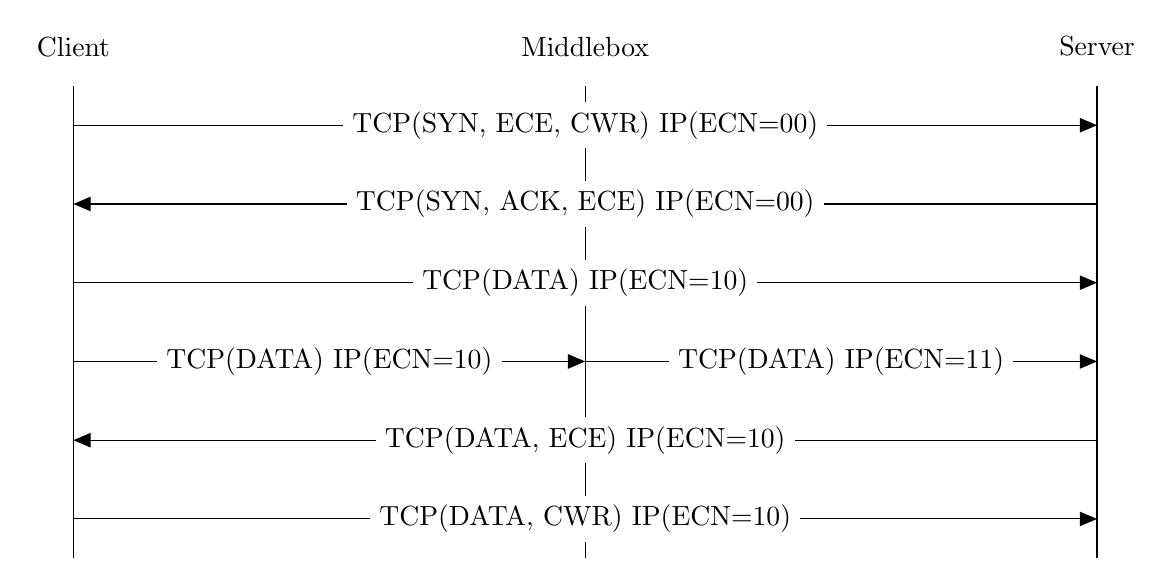
\begin{tikzpicture}
            
            \draw (0,0) -- (0, 6);
            \draw (6.5,0) -- (6.5, 6);
            \draw (13,0) -- (13, 6);
            \node at (0,6.5) {Client};
            \node at (6.5,6.5) {Middlebox};
            \node at (13,6.5) {Server};
            
            \draw [arrows={-triangle 45}]
            (0, 5.5) -- (13, 5.5) node [midway, fill=white, text centered]
            { TCP(SYN, ECE, CWR)  IP(ECN=00)};
            
            \draw [arrows={triangle 45-}]
            (0, 4.5) -- (13, 4.5) node [midway, fill=white, text centered]
            { TCP(SYN, ACK, ECE)  IP(ECN=00)};
            
            \draw [arrows={-triangle 45}]
            (0, 3.5) -- (13, 3.5) node [midway, fill=white, text centered]
            { TCP(DATA)  IP(ECN=10)};
            
            \draw [arrows={-triangle 45}]
            (0, 2.5) -- (6.5, 2.5) node [midway, fill=white, text centered]
            { TCP(DATA)  IP(ECN=10)};
            
            \draw [arrows={-triangle 45}]
            (6.5, 2.5) -- (13, 2.5) node [midway, fill=white, text centered]
            { TCP(DATA)  IP(ECN=11)};
            
            \draw [arrows={triangle 45-}]
            (0, 1.5) -- (13, 1.5) node [midway, fill=white, text centered]
            { TCP(DATA, ECE)  IP(ECN=10)};
            
            \draw [arrows={-triangle 45}]
            (0, 0.5) -- (13, 0.5) node [midway, fill=white, text centered]
            { TCP(DATA, CWR)  IP(ECN=10)};
            
            \end{tikzpicture}
        \caption{Diagrammatic representation of the operation of the ECN extension with TCP/IP with a congested link on the network, TCP acks have been omitted for the sake of brevity}
    \label{fig:ecn_tcp}
    \end{figure}
\end{center}
\section{ECN within UDP}

ECN is not directly used with UDP, the exact operation of ECN with UDP is deferred to the context of a higher layer protocol, such as RTP, or Quic, which utilise UDP as their transport substrate. In the following text, we discuss the operation of ECN within Quic, one of the protocols investigated in this paper. Quic introduced the notion of ECN support with an IETF draft \cite{johansson_ecn_2017} discussing its intended operation. Whilst Quic is still in development as a protocol (lacking an RFC ), we summarise the operation of UDP under Quic within the draft used within this paper (ietf-draft-29)

When ECN is utilised with Quic, the sender must first determine whether both the path and the end host support ECN marking. This is defined as whether ECT codepoints are not cleared on path, or packets setting ECT codepoints are dropped, as well as the end host being able to both view and set the ECN field on the IP header. This is achieved through sending early Quic packets marked with either ECT(0) or ECT(1). Assuming packets are recieved by the end host, the receivers response should contain an "ECN ACK Frame" containing counts of packets observed with ECT(0), ECT(1) or CE. Of which the sender must validate, to ensure that the path and host support ECN markings. Following this, the sender may continue to send ECT marked packets. If a sending host, receives an ECN Ack frame that increases the CE count. The sender is to reduce their congestion window, in a similar manner to as if a loss had occurred. In a similar manner to ECN under TCP/IP.

\section{ICMP Quotations}
\label{sec:icmp}

Introduced in RFC 792, it is required for some ICMP responses to quote the IP header and the first 8 bytes of associated data. In particular 'TTL exceeded in transit' ICMP responses, are required by the RFC to observe this behaviour. This allows for path level insight to the IP header, and specifically, insight into remarking behaviour of ECN codepoints from within the network. This mechanism is used extensively in the existing literature on network measurement. Additionally in RFC 1812 this behaviour is recommended to be extended to not just aspects of the packet header, but the entire IP packet, however \cite{noauthor_tracebox_nodate} notes that this behaviour is less commonly observed as to only being adopted by some major vendors of networking equipment. The general concept around using ICMP responses to gain path level insight into the network is through the implementation of a traceroute style utility. 

From a given end-host on the network, We begin through sending packets into the network with a Time to Live (TTL) of one. the TTL field of the IP header describes the lifetime of an IP packet. When an IP packet arrives at a router, it is to decrement the TTL by one. If the TTl reaches zero, the packet is to be dropped by the router, and an ICMP TTL exceeded response is to be sent containing at least the the first 8 bytes of the IP header. We in turn receive the ICMP TTL exceeded responses containing the the first 8 bytes of data that was sent. This can be inspected to determine whether particular modifications have occurred in transit, and roughly where on the network that this occurs. This process is then repeated for increasing TTL values such that the packet traverses further into the network. We typically stop this procedure when either the end host responds, or a given TTL value is reached. The process is summarised in figure \ref{fig:icmp}.

\begin{figure}[h!]

\centering
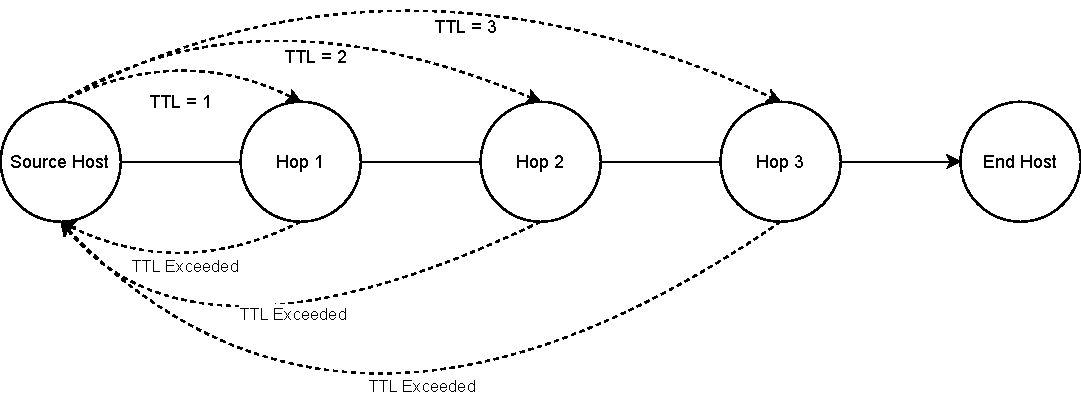
\includegraphics[width=14cm,keepaspectratio]{dissertation/images/icmp.pdf}
\caption{A diagrammatic representation of how ICMP quotations can be used to observe modifications to the IP header on the network path.}
\label{fig:icmp}
\end{figure}

\section{Previous Works}

There exists an extensive body of work on ECN measurement across the last two decades, in this subsection we present and evaluate previous contributions in the area.

\subsection{Measuring the state of ECN Readiness in clients and Servers}


There exists an extensive body of work on ECN measurement across the last two decades concerning the deployment of ECN within TCP. \cite{bauer_measuring_2011} measured the top one million web servers as ranked by the alexa top sites list, a collection of college and university based hosts and a collection of hosts intended for use with mobile devices. Measuring what fraction of hosts would negotiate ECN, additionally investigating whether middleboxes or routers on the network path were clearing ECT codepoints using an approach based on ICMP probes of the network as described in section \ref{sec:icmp}. From a collection of vantage points hosted in datacentres or university networks. The authors found that 94.8\% of hosts preserved the ECT codepoint across the network path. Additionally the authors utilised a robust approach to identify a given interface that may be responsible for remarking the ECN codepoint, additionally attributing this behaviour to a particular AS, we see a particular bias to earlier in the network path, however this should be expected, as given when ECN codepoints are remarked subsequent parts of the network path are unable to be evaluated. This paper primarily used the CE codepoint in its network measurements, hence does not investigate the possibility of differential treatment of the codepoints on the network. Additionally, this paper was produced before the advent of the Quic network protocol


\subsection{Is ECN Usable With UDP}

Additional studies have also concerned themselves with the deployment of UDP based protocols incorporating ECN. \cite{mcquistin_is_2015} investigated in the broader sense whether ECN was usable with UDP, through the evaluation of 2,500 NTP pool servers. Revealing that ECN had a minor impact on the reachability of NTP servers. The authors breifly examined, where on the path ECT(0) codepoints were removed from packets, through implementing traceroutes to given hosts. Sending TTL limited packets with increasing hop limits until a response from the intended hosts is recieved. The generated ICMP TTL exceeded responses being collected in the process. The authors identified that in the majority of cases ECT(0) codepoints do traverse the network. Furthermore, when ECT codepoints are stripped from packets, this occurs distantly from the host, with the responsible device being located on an AS boundary. The authors did not use a directly comparable approach for that of TCP connections against the same host, although the core focus of the study was in evaluating the usability of UDP.

\subsection{Exploring DSCP modification pathologies in the internet}

\cite{custura_exploring_2017} examined the wider traffic class byte. With a particular focus on the DSCP codepoint however the author discovers many different modification pathologies that in some cases effect ECN codepoints as well. In particular demonstrating a correlation between DSCP codepoint remarking and ECN remarking in many cases, suggesting that some routers erronously clear the ECN field as a consequence of continuing to use ToS semantics. However, this is not universal suggesting that not all ECN remarking behaviour is due to this. Furthermore the author investigates whether the transport protocol in use influences the DSCP modifications pathologies discussed in the paper. This analysis is not extended to the 3 ECN codepoints, for which the modification pathologies slightly differ as shown in the paper.

\subsection{PathSpider}

There also exists a collection of existing tools tailored for network measurement. PathSpider is one of these tools, it is intended active measurement to reveal impairments on the network path. PathSpider allows for connections to a given host to be carried out in the format of an A/B test to reveal a given characteristic of the host or network path. For instance revealing whether a given connection to a host fails when ECN is negotiated. However for the purposes of this paper the default configurations of PathSpider were deemed insufficient. PathSpider treats the network at large as a black box. That is, PathSpider is sufficient at signalling when a given condition occurs, for example, whether a given TCP segement marked with ECE results in a CWR in response. However this signalling is not extended to where on the network path that the impairment occurs is located. Additionally newer protocols that are of interest, such as Quic do not have existing plugins supporting their analysis.

\subsection{Tracebox}

Tracebox is another network path transparency tool. Tracebox is viewed as a spiritual successor to the widely used traceroute tool allowing the user to identify the existence and behaviour of certain devices on the network such as NATs through evaluating ICMP responses as mentioned in section \ref{sec:icmp} against the source packet and identifying modifications. Whilst tracebox does feature a programmatic interface in Lua it was deemed at insufficient in implementing a plugin for evaluating Quic. 

\subsection{Scamper}


\subsection{Scriptroute}





% discuss the history of the dscp and tos, and why might network operators interact with these aspects of the ip header

% ECN (Explicit Congestion Notification) provides a means for devices on the network path to signal impending congestion to end hosts, allowing them to reduce their sending rates before packet loss occurs. However, the deployment of ECN has been stiffled due to concerns with how the relevant markings on internet traffic interact with the wider network. Particularly in the case of firewalls. Interest in the deployment of ECN has increased over recent years, in particular around newer protcols such as Quic, for which a proposal to add ECN support to quic has been around since 2017.

% {{Discussion of the codepoints that ECN uses}}

% {{Discussion of how ecn works with TCP}}

% {{Discussion of how ECN is proposed to operate with Quic}}

% {{Discussion of ICMP quotations}}


%==================================================================================================================================
\addtocontents{toc}{\protect\setcounter{tocdepth}{2}}
\chapter{Analysis/Requirements}

The following chapter details the analysis of the problem domain. Documenting how the scope of the project was narrowed, informing the design and subsequent implementation phases of the project.

\section{General Problem}

\subsection{Detecting Removal of ECT codepoints}

To determine whether ECT marked packets are traversing the network, we refer to the description presented in Section \ref{sec:icmp}. Describing a process of sending packets with increasing TTL values, and collecting returned ICMP responses. Notably, as at least the IP header and the first 8 bytes of associated data with a given packet are returned within the ICMP quotation. This allows for the contents of the ECN field in particular to be observed as the packet traverses the network hop by hop.

% How do we figure out what is going on on the network -> ttl exceeded responses %

% Visualisation of packets traversing the network %

\subsection{Attributing ECT removal to a network interface or Autonomous System}

In attempting to attribute ECT modification a particular device on the network introduces a number of ambiguities. Consider the case of an arbitrary traceroute to a given end host

\begin{figure}[h!]

\centering
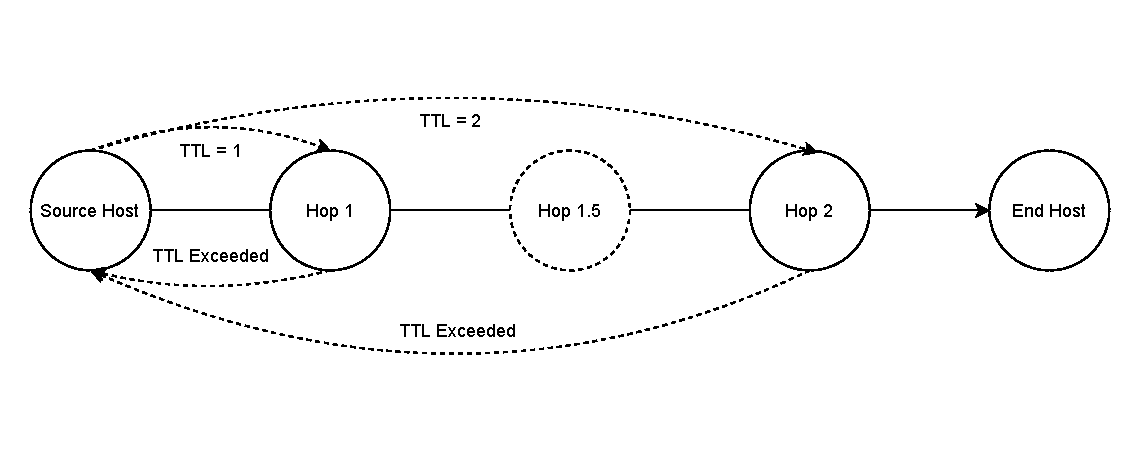
\includegraphics[width=14cm,keepaspectratio]{dissertation/images/ambig_icmp.pdf}
\caption{A diagrammatic representation of how ambiguities may arise with attributing ECT removal to a particular device on the network.}
\label{fig:icmp}
\end{figure}

\subsection{Generalizing to the wider network}

As is generally seen as good scientific practice, we wish to obtain results that are on the whole generalizable. In the context of this paper, we seek to generalize the treatment of ECT codepoints within the wider network. For example, if we opted to obtain measurements from a singular host or vantage point on the network, we introduce a vulnerability to a particular device located close to the Host on the network that may erroneously clear ECT codepoints, potentially biasing results. Additionally, geographically close hosts, or hosts that share the same underlying Internet Service Provider (ISP). May share much of the same network level path to particular end hosts, hence are vulnerable to the same issues presented with collecting data from a singular vantage point on the network. Additionally, when we measure the network itself. We wish to ensure that a wide number of paths on the network are tested, and that these paths are generally representative of usage of the network.


\section{Requirements}

With respect to the presented general problem, we highlight the existence of several requirements that were deduced during the course of the project and subsequently prioritised using the MoSCoW method to guide the development of project within the defined time constraints. Ensuring that the project met the initial criteria, producing data that would answer the questions posed.

\subsection{Functional Requirements}

\begin{itemize}
    \item 
\end{itemize}



\subsection{Non-functional Requirements}

\begin{itemize}
    \item The developed tool should be readily deployable on both x86, and Arm based computers, to ensure that the tool is convenient to deploy by end users
\end{itemize}

\section{Summary}

In this chapter we have discussed the general problem domain around active network measurement with respect to ECN, we have discussed the rationale behind the general approach to measuring where on the network path ECN codepoints are stripped.




%==================================================================================================================================
\chapter{Design}
\label{chap:design}

Given the nature of the topic, we identify two high level aspects of design, that of the network analysis tool required to gather suitable measurements from the network, and the experimental design itself, to ensure that the measurements we gather from the network are both robust and are capable of answering the questions proposed in {{Where aims are proposed}}

\section{Tooling}

what we need to measure -> design of experiemnt
how we measure it -> design of tool
where deploy in many places -> choice of aws and participant locations

\subsection{Network analysis tool}
{{Create a graph with graphviz to visualise how tool components interact with eachother and the wider network ie. system architecture diagram}}

{{Small discussion of the high level components of the tool}}
{{Traffic generator}}
{{Traffic modification}}
{{Traffic capture}}

\section{Experimental Design}

{{3 server populations to gather a representative sample of the network; Overview of dataset}}
{{Tool operates through the dataset over a space of 48 hours, over a period of two weeks}}


{{Collection of vantage points, AWS hosts, at least one in each continent that AWS operates}}
{{Collection of residential hosts through an ethics approved study}}


{{Overview of specifics of traffic generated}}
{{What types of connection for each host}}
{{ECT markings on each connection}}


%==================================================================================================================================
\chapter{Implementation}

discuss issues with deployment
firewall issues
Issue relating to TCP and NTP

aws deployment -> terraform

{{Overview of each component}}

{{Traffifc modifier}}
{{Preffered over iptables rules -> programmatic access to packets as opposed to generic over arching rules}}

{{Traffic capturer}}
{{Basically just a mention that libpcap was used}}

{{Traffic generator}}
{{Overview of lsquic: fixed on draft 29}}
{{Overview of TCP on path traceroutes}}

%==================================================================================================================================
\chapter{Results} 

As discussed in \autoref{chap:introduction} we seek to investigate Where ECT codepoints are removed from network traffic on the network. This is inherently, a very broad topic. In order to focus our discussions, we select the following topics to investigate

{{Each of the following sections with a justification for being in the paper}}

\section{An Overview of ECN adoption}

We want, a table on ECN negotiated by web server host
place this as an additional data point on ecn adoption across other hosts, baur et al, medina etc etc


\section{Are ECT code points stripped during TCP connections?}

Given the methodology noted in chapter n, and the subsequent implementation of the network analyis tool this allowed us to investigate whether ect codepoints are removed during a TCP connections.

From the webserver hosts we discovered that across our experiment, ect code points were modified on approx x\% of connections, tableN details the number of observed, this appears (in)consistent with measurements  from etc etc

\subsection{Where are ECT codepoints removed during TCP connections}

To understand where on the connection ect codepoints are removed we use our trace data obtained during TCP connections and produce a cumulative density function against number of interface hops on path against the total number of interface hops on the path (ie) the maximum ttl recorded from the vantage point when the host repsonds to the tracerouted request.

The CDF shows extensive modification in the in the latter half of the network path that was traversed, notably across the network core. And network hops close to the end host

\^ the above may be replaced with a similar graph to the paper "DSCP modification pathologies in mobile edge networks"

\section{Are ECT code points treated consistently by network devices}

we want a table breaking down, reachability of a given set of hosts, as well as incorporating


\section{Does the Network protocol version influence modification pathologies}

Take web hosts that operate over both IPv4 and IPv6, could make some measure of how similar the paths
are for given hosts, or just in the general sense that the hosts are the same


\section{Does the transport protocol influence ECT modification pathologies?}

TCP and udp enabled host on the same port -> use dns servers
Unsure on what statistical test to use


\section{A Quick overview of Quic}

Quic, a relatively new transport protocol introduced ECN as part of Draft, we investigate the extent to which ECN has been deployed with current quic implementations



\subsection{An overview of ECN adoption under Quic}

Across our dataset of webserver hosts, we found that no webserver hosts negotatiated ECN, with ~40 hosts negotiating QUic at all, we define a host that negotiated ECN as doing one of the following. Marking responses with ECT codepoints, or responsing with packets that contain ECT ack frames as defined in RFCxyz. We attribute this lack of ECN adoption to the immatirity of the protocol itself.

\subsection{An overview of ECT modfications under quic}

Similarily to \\tcphosts we produce a cumulative density function to visualize where on path ECT depoints are modified for connections against hosts operating over Quic. We see differences in the modification pathologies from TCPconnections to Quic connections. That is, we see a particular bias towards the end of the path for hosts operating over Quic

CDF representing where (as a ratio) on path codepoints are cleared


\section{Other Notable Behaviours}

{{Brief mention of ECT marked ICMP responses}}



%==================================================================================================================================
\chapter{Conclusion}    
\section{Summary}


\section{Future Work}

Whilst it is believed that the experiment was successful in testing a variety of network pathways from numerous vantage points, we accept that there were limitations presented as a result of sourcing participants from a limited geographic distribution.

Furthermore, as the deployment of Quic progresses, gathering data from a wider collection of hosts would be desirable to attain a more general understanding of how ECN under Quic interacts with the wider network.


%==================================================================================================================================
%
% 
%==================================================================================================================================
%  APPENDICES  

\begin{appendices}

\chapter{Introduction and debrief scripts}

\section{Introduction Script}
\section{Debrief Script}

\end{appendices}

%==================================================================================================================================
%   BIBLIOGRAPHY   

% The bibliography style is abbrvnat
% The bibliography always appears last, after the appendices.

\bibliographystyle{abbrvnat}

\bibliography{l4proj}

\end{document}
